\documentclass[a4paper,12pt]{article}
\usepackage{czech}
\usepackage[utf8]{inputenc}
\usepackage{a4wide}
\usepackage[dvipdfm]{graphicx}
\usepackage{graphics}
\usepackage{indentfirst}
\usepackage{fancyhdr}
\usepackage{setspace}
\usepackage{amsmath}
\usepackage{amssymb}
\usepackage{epsfig}

%%\usepackage{nopageno}
%%\usepackage{txfonts}
\usepackage[usenames]{color}


\begin{document}
\newcommand{\st}{^{\circ}}

\section{Úkol}

\begin{enumerate}
\item Změřte absorpční spektrum roztoků kalmagitu s koncentracemi $c_0, c_{0/2}, c_{0/4}$ při pH = 10 v celém oboru viditelného světla. Zpracujte graficky. Pro tři vybrané vlnové délky zkontrolujte platnost Beerova zákona. Zpracujte graficky.
\item Měření z bodu 1. pro koncentraci $c_{0/2}$ doplňte proměřením dvou roztoků kalmagitu téže koncentrace, které navíc obsahují $5\cdot 10^{-5}$ mol/l a $25\cdot 10^{-5}$ mol/l síranu hořečnatého MgSO4. Získaná tři spektra zpracujte graficky, určete isobestické body.
\item Proveďte odhad chyby transmitance a určete chybu nepřímého měření absorpčního koeficientu.
\end{enumerate}

\section{Teorie}
\subsection{Transmitance}
Transmitance je definována vztahem
\begin{eqnarray}
\theta = \Phi_t/\Phi_0,
\end{eqnarray}
kde $\Phi_t$ resp. $\Phi_0$ je prošlý resp. na látku dopadající světelný tok. Pokud vypustíme ztráry na odrazech získáme $\theta_i$, což značí vnitřní transmitanci. 
Její doplněk do jedničky se nazývá absorptance.

\subsection{Lambertův zákon}
Lambertův uákon říká, že vnitřní transmitance v látce se chová dle rovnice
\begin{eqnarray}
\theta_i=10^{\kappa l}=\mbox{e}^{\kappa_nl},
\end{eqnarray}
kde $\kappa$ a $\kappa_n$ jsou absorbční koeficienty.

\subsection{Absorbance}
Absorbance je definována vztahem
\begin{eqnarray}
A=\kappa l
\end{eqnarray}

\subsection{Lambert-Beerův zákon}
Lambert-Beerův zákon říká, že
\begin{eqnarray}
\theta_i=10^{\varepsilon cl},
\end{eqnarray}
kde $\varepsilon$ je molární absorbční koeficint a $c$ molární koncentrace roztoku.

Pro více neovlivňujících se látek platí navíc vztah pro absorbanci
\begin{eqnarray}
A=l\sum\varepsilon_ic_i.
\end{eqnarray}

\section{Měření}
Nejprve jsem si připravil roztoky, které se budou měřit. Jejich složení je shrnuto v tabulce \ref{TR}. Roztoky jsem přelil do připravených kyvet, jejiž tloušťka byla 
$l=(1.000 \pm 0.001)$ cm.

\begin{table}
$$
\begin{array}{|l|c|c|c|c|c|}
\hline
&   c_0&    c_0/2&    c_0/4&    c_0/2\cdot c_{MgSO4}& c_0/2\cdot 5c_{MgSO4} \\ \hline
\mbox{kalagnit}&    5&  2.5&  1.25& 2.5&    2.5 \\ \hline
\mbox{MgSO4}&   0&  0&  0&  1&  5 \\ \hline
\mbox{pufr}&    1&  1&  1&  1&  1 \\ \hline
\mbox{H2O}& 4&  6.5&    7.75&   5.5&    1.5 \\ \hline
\end{array}
$$
\caption{Solžení měřených rozoků}
\label{TR}
\end{table}

Následně jsem seřídíl spektrofotometr a v závislosti na vlnové délce použitého světla jsem proměřil vnitřní transmitanci. Výsledky jsou v tabulce \ref{TM}. Výsledné závislosti 
jsou vidět na obrázcích \ref{g1} a \ref{g2}. Z grafu \ref{g2} jsem následně určil isobestické body
\begin{eqnarray}
\lambda_0=410 \mbox{nm} \\
\lambda_1=561 \mbox{nm}
\end{eqnarray}

\begin{table}
$$
\begin{array}{|c|c|c|c|c|c|}
\hline
\lambda/\mbox{nm}&   100\theta_{c_0}&   100\theta_{c_0/2}&    100\theta{c_0/4}&    100\theta{c_0/2\cdot c_{MgSO4}}& 100\theta{c_0/2\cdot 5c_{MgSO4}} \\ \hline
400&    47& 72& 87& 72& 75 \\ \hline
420&    54& 76& 88& 73& 73 \\ \hline
440&    56& 77& 89& 69& 68 \\ \hline
460&    55& 75& 88& 61& 60 \\ \hline
480&    50& 72& 86& 51& 49 \\ \hline
500&    40& 66& 82& 37& 35 \\ \hline
520&    26& 55& 76& 29& 26 \\ \hline
540&    16& 45& 70& 27& 26 \\ \hline
560&    11& 41& 68& 39& 40 \\ \hline
580&    8&  36& 66& 58& 62 \\ \hline
600&    6&  34& 66& 72& 81 \\ \hline
620&    6&  34& 68& 79& 90 \\ \hline
640&    9&  38& 71& 82& 94 \\ \hline
660&    20& 52& 78& 85& 96 \\ \hline
680&    46& 72& 88& 91& 98 \\ \hline
700&    72& 87& 95& 96& 99 \\ \hline
\end{array}
$$
\caption{Neměření hodnoty vnitřní transmitance v závislosti na vlnpvé délce}
\label{TM}
\end{table}

Pro vlnové délky 440, 540 a 640 nm jsem z hodnoty $\theta_{c_0}$ vypočetl $\varepsilon$ 
pro danou vlnovou délku.
\begin{eqnarray}
lc_0\varepsilon{440}=0.25181 \\
lc_0\varepsilon{540}=0.79588\\
lc_0\varepsilon{640}=1.04576\\
\end{eqnarray}
Dále dosadil do Lambert-Beerova zákonu abych dopočítal teoretické hodnoty s určil rozdíl odhodnot naměřených.
\begin{eqnarray}
100\Delta\theta_{c_0/2}(440)=-2 \\
100\Delta\theta_{c_0/4}(440)=-2 \\
100\Delta\theta_{c_0/2}(540)=-5 \\
100\Delta\theta_{c_0/4}(540)=-7 \\
100\Delta\theta_{c_0/2}(640)=-8 \\
100\Delta\theta_{c_0/4}(640)=-16 \\
\end{eqnarray}


\begin{figure}
% GNUPLOT: LaTeX picture with Postscript
\begingroup
  \makeatletter
  \providecommand\color[2][]{%
    \GenericError{(gnuplot) \space\space\space\@spaces}{%
      Package color not loaded in conjunction with
      terminal option `colourtext'%
    }{See the gnuplot documentation for explanation.%
    }{Either use 'blacktext' in gnuplot or load the package
      color.sty in LaTeX.}%
    \renewcommand\color[2][]{}%
  }%
  \providecommand\includegraphics[2][]{%
    \GenericError{(gnuplot) \space\space\space\@spaces}{%
      Package graphicx or graphics not loaded%
    }{See the gnuplot documentation for explanation.%
    }{The gnuplot epslatex terminal needs graphicx.sty or graphics.sty.}%
    \renewcommand\includegraphics[2][]{}%
  }%
  \providecommand\rotatebox[2]{#2}%
  \@ifundefined{ifGPcolor}{%
    \newif\ifGPcolor
    \GPcolorfalse
  }{}%
  \@ifundefined{ifGPblacktext}{%
    \newif\ifGPblacktext
    \GPblacktexttrue
  }{}%
  % define a \g@addto@macro without @ in the name:
  \let\gplgaddtomacro\g@addto@macro
  % define empty templates for all commands taking text:
  \gdef\gplbacktext{}%
  \gdef\gplfronttext{}%
  \makeatother
  \ifGPblacktext
    % no textcolor at all
    \def\colorrgb#1{}%
    \def\colorgray#1{}%
  \else
    % gray or color?
    \ifGPcolor
      \def\colorrgb#1{\color[rgb]{#1}}%
      \def\colorgray#1{\color[gray]{#1}}%
      \expandafter\def\csname LTw\endcsname{\color{white}}%
      \expandafter\def\csname LTb\endcsname{\color{black}}%
      \expandafter\def\csname LTa\endcsname{\color{black}}%
      \expandafter\def\csname LT0\endcsname{\color[rgb]{1,0,0}}%
      \expandafter\def\csname LT1\endcsname{\color[rgb]{0,1,0}}%
      \expandafter\def\csname LT2\endcsname{\color[rgb]{0,0,1}}%
      \expandafter\def\csname LT3\endcsname{\color[rgb]{1,0,1}}%
      \expandafter\def\csname LT4\endcsname{\color[rgb]{0,1,1}}%
      \expandafter\def\csname LT5\endcsname{\color[rgb]{1,1,0}}%
      \expandafter\def\csname LT6\endcsname{\color[rgb]{0,0,0}}%
      \expandafter\def\csname LT7\endcsname{\color[rgb]{1,0.3,0}}%
      \expandafter\def\csname LT8\endcsname{\color[rgb]{0.5,0.5,0.5}}%
    \else
      % gray
      \def\colorrgb#1{\color{black}}%
      \def\colorgray#1{\color[gray]{#1}}%
      \expandafter\def\csname LTw\endcsname{\color{white}}%
      \expandafter\def\csname LTb\endcsname{\color{black}}%
      \expandafter\def\csname LTa\endcsname{\color{black}}%
      \expandafter\def\csname LT0\endcsname{\color{black}}%
      \expandafter\def\csname LT1\endcsname{\color{black}}%
      \expandafter\def\csname LT2\endcsname{\color{black}}%
      \expandafter\def\csname LT3\endcsname{\color{black}}%
      \expandafter\def\csname LT4\endcsname{\color{black}}%
      \expandafter\def\csname LT5\endcsname{\color{black}}%
      \expandafter\def\csname LT6\endcsname{\color{black}}%
      \expandafter\def\csname LT7\endcsname{\color{black}}%
      \expandafter\def\csname LT8\endcsname{\color{black}}%
    \fi
  \fi
  \setlength{\unitlength}{0.0500bp}%
  \begin{picture}(7200.00,5040.00)%
    \gplgaddtomacro\gplbacktext{%
      \csname LTb\endcsname%
      \put(1210,704){\makebox(0,0)[r]{\strut{} 700}}%
      \put(1210,1074){\makebox(0,0)[r]{\strut{} 800}}%
      \put(1210,1444){\makebox(0,0)[r]{\strut{} 900}}%
      \put(1210,1814){\makebox(0,0)[r]{\strut{} 1000}}%
      \put(1210,2184){\makebox(0,0)[r]{\strut{} 1100}}%
      \put(1210,2554){\makebox(0,0)[r]{\strut{} 1200}}%
      \put(1210,2925){\makebox(0,0)[r]{\strut{} 1300}}%
      \put(1210,3295){\makebox(0,0)[r]{\strut{} 1400}}%
      \put(1210,3665){\makebox(0,0)[r]{\strut{} 1500}}%
      \put(1210,4035){\makebox(0,0)[r]{\strut{} 1600}}%
      \put(1210,4405){\makebox(0,0)[r]{\strut{} 1700}}%
      \put(1210,4775){\makebox(0,0)[r]{\strut{} 1800}}%
      \put(1342,484){\makebox(0,0){\strut{} 0}}%
      \put(2263,484){\makebox(0,0){\strut{} 0.5}}%
      \put(3184,484){\makebox(0,0){\strut{} 1}}%
      \put(4105,484){\makebox(0,0){\strut{} 1.5}}%
      \put(5027,484){\makebox(0,0){\strut{} 2}}%
      \put(5948,484){\makebox(0,0){\strut{} 2.5}}%
      \put(6869,484){\makebox(0,0){\strut{} 3}}%
      \put(308,2739){\rotatebox{-270}{\makebox(0,0){\strut{}$h$/keV$\cdot$m$^{-1}$}}}%
      \put(4105,154){\makebox(0,0){\strut{}$x$/cm}}%
    }%
    \gplgaddtomacro\gplfronttext{%
    }%
    \gplbacktext
    \put(0,0){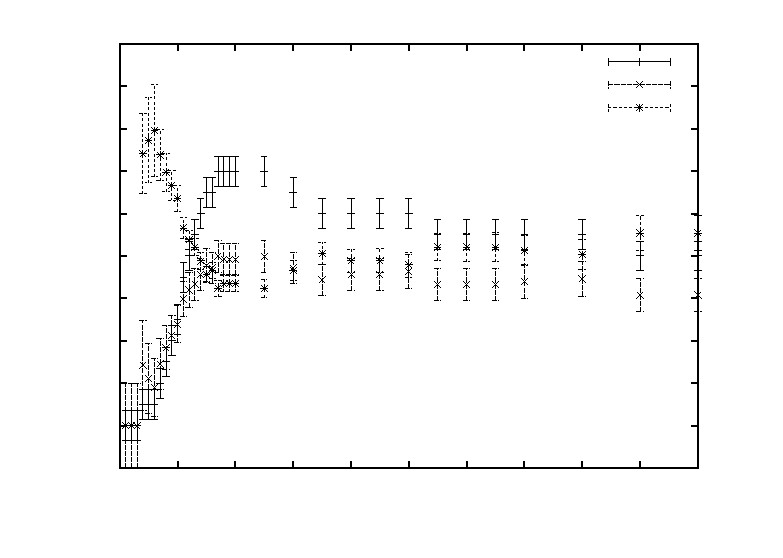
\includegraphics{g1}}%
    \gplfronttext
  \end{picture}%
\endgroup

\caption{Graf závislosti transmitance na vlnové délce}
\label{g1}
\end{figure}

\begin{figure}
% GNUPLOT: LaTeX picture with Postscript
\begingroup
  \makeatletter
  \providecommand\color[2][]{%
    \GenericError{(gnuplot) \space\space\space\@spaces}{%
      Package color not loaded in conjunction with
      terminal option `colourtext'%
    }{See the gnuplot documentation for explanation.%
    }{Either use 'blacktext' in gnuplot or load the package
      color.sty in LaTeX.}%
    \renewcommand\color[2][]{}%
  }%
  \providecommand\includegraphics[2][]{%
    \GenericError{(gnuplot) \space\space\space\@spaces}{%
      Package graphicx or graphics not loaded%
    }{See the gnuplot documentation for explanation.%
    }{The gnuplot epslatex terminal needs graphicx.sty or graphics.sty.}%
    \renewcommand\includegraphics[2][]{}%
  }%
  \providecommand\rotatebox[2]{#2}%
  \@ifundefined{ifGPcolor}{%
    \newif\ifGPcolor
    \GPcolorfalse
  }{}%
  \@ifundefined{ifGPblacktext}{%
    \newif\ifGPblacktext
    \GPblacktexttrue
  }{}%
  % define a \g@addto@macro without @ in the name:
  \let\gplgaddtomacro\g@addto@macro
  % define empty templates for all commands taking text:
  \gdef\gplbacktext{}%
  \gdef\gplfronttext{}%
  \makeatother
  \ifGPblacktext
    % no textcolor at all
    \def\colorrgb#1{}%
    \def\colorgray#1{}%
  \else
    % gray or color?
    \ifGPcolor
      \def\colorrgb#1{\color[rgb]{#1}}%
      \def\colorgray#1{\color[gray]{#1}}%
      \expandafter\def\csname LTw\endcsname{\color{white}}%
      \expandafter\def\csname LTb\endcsname{\color{black}}%
      \expandafter\def\csname LTa\endcsname{\color{black}}%
      \expandafter\def\csname LT0\endcsname{\color[rgb]{1,0,0}}%
      \expandafter\def\csname LT1\endcsname{\color[rgb]{0,1,0}}%
      \expandafter\def\csname LT2\endcsname{\color[rgb]{0,0,1}}%
      \expandafter\def\csname LT3\endcsname{\color[rgb]{1,0,1}}%
      \expandafter\def\csname LT4\endcsname{\color[rgb]{0,1,1}}%
      \expandafter\def\csname LT5\endcsname{\color[rgb]{1,1,0}}%
      \expandafter\def\csname LT6\endcsname{\color[rgb]{0,0,0}}%
      \expandafter\def\csname LT7\endcsname{\color[rgb]{1,0.3,0}}%
      \expandafter\def\csname LT8\endcsname{\color[rgb]{0.5,0.5,0.5}}%
    \else
      % gray
      \def\colorrgb#1{\color{black}}%
      \def\colorgray#1{\color[gray]{#1}}%
      \expandafter\def\csname LTw\endcsname{\color{white}}%
      \expandafter\def\csname LTb\endcsname{\color{black}}%
      \expandafter\def\csname LTa\endcsname{\color{black}}%
      \expandafter\def\csname LT0\endcsname{\color{black}}%
      \expandafter\def\csname LT1\endcsname{\color{black}}%
      \expandafter\def\csname LT2\endcsname{\color{black}}%
      \expandafter\def\csname LT3\endcsname{\color{black}}%
      \expandafter\def\csname LT4\endcsname{\color{black}}%
      \expandafter\def\csname LT5\endcsname{\color{black}}%
      \expandafter\def\csname LT6\endcsname{\color{black}}%
      \expandafter\def\csname LT7\endcsname{\color{black}}%
      \expandafter\def\csname LT8\endcsname{\color{black}}%
    \fi
  \fi
  \setlength{\unitlength}{0.0500bp}%
  \begin{picture}(7200.00,5040.00)%
    \gplgaddtomacro\gplbacktext{%
      \csname LTb\endcsname%
      \put(814,704){\makebox(0,0)[r]{\strut{} 0}}%
      \put(814,1213){\makebox(0,0)[r]{\strut{} 1}}%
      \put(814,1722){\makebox(0,0)[r]{\strut{} 2}}%
      \put(814,2231){\makebox(0,0)[r]{\strut{} 3}}%
      \put(814,2740){\makebox(0,0)[r]{\strut{} 4}}%
      \put(814,3248){\makebox(0,0)[r]{\strut{} 5}}%
      \put(814,3757){\makebox(0,0)[r]{\strut{} 6}}%
      \put(814,4266){\makebox(0,0)[r]{\strut{} 7}}%
      \put(814,4775){\makebox(0,0)[r]{\strut{} 8}}%
      \put(946,484){\makebox(0,0){\strut{} 0}}%
      \put(1404,484){\makebox(0,0){\strut{} 0.1}}%
      \put(1863,484){\makebox(0,0){\strut{} 0.2}}%
      \put(2321,484){\makebox(0,0){\strut{} 0.3}}%
      \put(2780,484){\makebox(0,0){\strut{} 0.4}}%
      \put(3238,484){\makebox(0,0){\strut{} 0.5}}%
      \put(3697,484){\makebox(0,0){\strut{} 0.6}}%
      \put(4155,484){\makebox(0,0){\strut{} 0.7}}%
      \put(4614,484){\makebox(0,0){\strut{} 0.8}}%
      \put(5072,484){\makebox(0,0){\strut{} 0.9}}%
      \put(5531,484){\makebox(0,0){\strut{} 1}}%
      \put(5989,484){\makebox(0,0){\strut{} 1.1}}%
      \put(6121,1043){\makebox(0,0)[l]{\strut{} 56}}%
      \put(6121,1722){\makebox(0,0)[l]{\strut{} 58}}%
      \put(6121,2400){\makebox(0,0)[l]{\strut{} 60}}%
      \put(6121,3079){\makebox(0,0)[l]{\strut{} 62}}%
      \put(6121,3757){\makebox(0,0)[l]{\strut{} 64}}%
      \put(6121,4436){\makebox(0,0)[l]{\strut{} 66}}%
      \put(308,2739){\rotatebox{-270}{\makebox(0,0){\strut{}$C/\mu$F}}}%
      \put(6758,2739){\rotatebox{-270}{\makebox(0,0){\strut{}$\tau/$s}}}%
      \put(3467,154){\makebox(0,0){\strut{}$I/$mA}}%
    }%
    \gplgaddtomacro\gplfronttext{%
      \csname LTb\endcsname%
      \put(5002,1317){\makebox(0,0)[r]{\strut{}$C$}}%
      \csname LTb\endcsname%
      \put(5002,1097){\makebox(0,0)[r]{\strut{}$7.72\cdot10^{-3}\{I\}$}}%
      \csname LTb\endcsname%
      \put(5002,877){\makebox(0,0)[r]{\strut{}$\tau$}}%
    }%
    \gplbacktext
    \put(0,0){\includegraphics{g2}}%
    \gplfronttext
  \end{picture}%
\endgroup

\caption{Graf závislosti transmitance na vlnové délce}
\label{g2}
\end{figure}

Měřící přístroj měj třidu přesnosti jedna, což odpovídá chybě jedné setiny u 
vnitřní transmitance. Vlnová délka byla určena s přesností v řádu procent. Vliv odrazů a vody byl díky metodě měření zanedbatelný. Chyba u šířky kyvety byla o dva řády nižší, a proto ji můžeme 
zanedbat. Chyba absorbčního koeficientu je dle \cite{chyba}
\begin{eqnarray}
\sigma_A=-\frac{\sigma_\theta}{\theta \ln 10}
\end{eqnarray}

\section{Diskuze}
Naměřené hodnoty v rámci chyby splňují teoretické předpoklady. Odchylka od teoretických 
hodnot sice s vlnovou délkou rostla, ale to bylo nejspíše způsobeno velkou relativní chybou vnitřní transmitance při měření malých hodnot. Při výpočtu $\varepsilon$ z hodnot prp nižší koncentrace by byla chyba výrazně nižší.

Co se týče příměsi, tak na grafu \ref{g2} jsou dobře vidět dva isobestické body. U prvního se projevila větší chyba způsobená měřením v oblasti nižšího výkonu rtuťové výbojky.

\section{Závěr}
Změřil jsem absorbční spektrum kalagmitu o různé koncentraci. Výsledky jsou v tabulce \ref{TM} a na obrázku \ref{g1}. Pro hodnoty 440, 540 a 640 nm jsem ověřil platnost Lambert-Beerova zákona. \\
Měření jsem doplnil roztokem s příměsí MgSO4. Výsledky jsou v tabulce \ref{TM} a na obrázku \ref{g2}. Určil jsem isobestické body
\begin{eqnarray}
\lambda_0=410 \mbox{nm} \\
\lambda_1=561 \mbox{nm}
\end{eqnarray}

Provedl jsem odhad chyby transmitance a vypočetl chybu absorbčního koeficientu
\begin{eqnarray}
\sigma_A=-\frac{\sigma_\theta}{\theta \ln 10}
\end{eqnarray}

\begin{thebibliography}{5}
	\bibitem{text} \textbf{Studijní text na praktikum III} \\http://physics.mff.cuni.cz/vyuka/zfp/txt\_317.htm (20. 4. 2012)
	\bibitem{text2} \textbf{Studijní text na praktikum III} \\http://physics.mff.cuni.cz/vyuka/zfp/mereni\_317.htm (20. 4. 2012)
    \bibitem{chyba} \emph{J. Englich}: \textbf{Zpracování výsldků fyzikálních měření} \\ LS 1999/2000
    \bibitem{maly} \emph{prof. RNDr. Petr Malý , DrSc.}: \textbf{Optika}\\Univerzita Karlova v Praze, Nakladatelství Karolinum 2008, první vydání
\end{thebibliography}






\end{document}
